\section{Design of the backend framework}\label{sec:design}

\subsection{Principles}\label{sec:design-principles}

Six rules were fixed before any code was written, and the rest of this
paper is largely a description of how they were kept. First, the
\numpy\ path is byte-identical to the previous version of \galpy. Every
backend helper is a strict pass-through when the active array library is
\numpy, such that migrated code written as \texttt{xp.sqrt(x)}, where
\texttt{xp} is the resolved namespace, runs the identical \numpy\ function
on the identical object. This rule is enforced by tests and, for each
PR, by comparing checksums of outputs between a checkout with and one
without the change. Where the \numpy\ result did change, this was
flagged and approved; there are three such places, discussed where they
arise. Second, the interface is unchanged: the same classes, methods,
and keywords, with the backend determined by the arrays that are passed
in. Third, \galpy's code is written against a backend-agnostic array
namespace, with backend-specific code confined to the \texttt{galpy.backend}
subpackage and never written as \texttt{if backend == 'jax'} inside the
physics. Fourth, \galpy\ uses the basic array operations of \jax\ and
\torch\ and little else; the numerical methods that \scipy\ supplies on
the \numpy\ path---special functions, root finding, quadrature,
interpolation, sampling---are implemented in \texttt{galpy.backend} and
tested against \scipy\ and against arbitrary-precision references,
rather than taken from the frameworks' own, uneven, \scipy-like
modules. Fifth, \galpy\ never compiles anything itself: the code is
written to be traceable by \texttt{jax.jit} and \texttt{torch.compile},
and the user decides what to compile. Sixth, the existing test suite,
run under every backend with the same tolerances, is the acceptance
test.

\subsection{Choosing a backend}\label{sec:design-choosing}

The backend follows the data. A \galpy\ function that receives a \jax\
array or a \torch\ tensor computes with that framework and returns an
array of the same kind; a function that receives \numpy\ arrays or
\python\ scalars computes with \numpy\ as before. Thus, the radial force
of the standard Milky-Way model is evaluated on a \jax\ array as
\begin{code}
from galpy.potential import MWPotential2014, evaluateRforces
R= jnp.linspace(0.5,2.,1001)
FR= evaluateRforces(MWPotential2014,R,0.) # a jax array, on R's device
\end{code}
without any further instruction, and with a \torch\ tensor the same
call returns a tensor. When there is no array to dispatch on, as when
a user sets up an \orb\ instance from \python\ floats, the default
backend is used; it is \numpy\ unless a different one is set in the
configuration file or through a context manager,
\begin{code}
import galpy.backend
with galpy.backend.use('jax'):
    o= Orbit([1.,0.1,1.1,0.,0.05,0.]) # initial condition becomes a jax array
    o.integrate(ts,MWPotential2014)   # ... and the orbit is integrated in jax
\end{code}
The resolution order is therefore: an explicit \texttt{xp=} argument,
the array arguments, the context or configured default, and finally
\numpy. The context manager also accepts \texttt{force=True}, which makes
the default take precedence over the data; this is what the test suite
uses to run \galpy's existing tests, written with \numpy\ inputs, under
a different backend, and it is not meant for production code.

Backend arrays go in and come out, but a few conventions are needed at
the edges. \galpy\ computes in double precision, and its internal
constants are \python\ floats, such that under \torch, whose default
is single precision, \galpy\ enters a double-precision default for the
duration of a call; a user's single-precision tensor stays single
precision in and out. Outputs that are scalars in the \numpy\ sense,
such as a single potential value for scalar inputs under a forced
backend, are returned as \numpy\ values, because \astropy\ units cannot
wrap a backend array. Units are handled outside the backend layer: a
\texttt{Quantity} input is converted to \galpy's internal units by the
existing unit-handling decorators before it reaches the backend code,
and a \texttt{Quantity} output is built from the result afterwards. A
potential parameter that is given as a backend array carries no units
and is taken to be in internal units already; this is what makes it
possible to differentiate with respect to it. \texttt{Quantity} objects
cannot be traced by \texttt{jax.jit}, and the use of units inside a
compiled program is therefore not supported (this accounts for three of
the six tests that remain in the ledger of
\sectionname~\ref{sec:process-ledger}).

\subsection{Backend-agnostic code}\label{sec:design-agnostic}

Every migrated compute method starts by resolving the array namespace
from its coordinate arguments and then uses only that namespace,
\begin{code}
def _evaluate(self,R,z,phi=0.,t=0.):
    xp= get_namespace(R,z,phi,t)
    return -self._amp/xp.sqrt(R**2+z**2+self._b2)
\end{code}
The namespace is the plain \numpy\ module for \numpy\ data,
\texttt{jax.numpy} for \jax\ arrays, and the array-API-compatible view of
\torch\ for tensors, obtained through the \texttt{array-api-compat}
package. This is the entire change for the majority of \galpy's
potentials, which are elementary functions of the coordinates; the
work is in the remainder, where \scipy\ or \numpy-specific functions
were used, and that work is described in the module sections. The
dispatch costs about $3\,\mu$s per call when run eagerly and nothing
under compilation, where it is resolved at trace time.

The dispatch is placed at \galpy's private compute layer
(\texttt{\_evaluate}, \texttt{\_Rforce}, and so on), such that the public
methods, their unit handling, and their documentation are untouched. The
public entry points carry one new decorator,
\texttt{@backend\_input('R','z','phi','t')}, that declares which of the
arguments are coordinates. The decorator coerces the declared arguments,
and only those, onto the active namespace, whether they are passed
positionally or by keyword; derivative orders, flags, masses, option
strings, and grids are left alone. It also resolves a single device for
the call from the first backend array it finds, such that a \python\
scalar passed alongside a GPU array does not end up on the host. On
\numpy\ data the decorator is a no-op. The central coercion matters
more than it might appear: \torch, unlike \jax, rejects \python\ scalars
in most tensor operations, and about two thousand of the tests that
failed under \torch\ when the backends were first run failed for this
reason alone. Coordinate transformations in \texttt{galpy.util.coords}
follow a similar pattern, where a marker decorator opts a migrated
function into framework-preserving scalar promotion, such that functions
could be migrated one at a time.

\subsection{Numerical building blocks}\label{sec:design-numerics}

\galpy's \numpy\ code uses \scipy\ for special functions, root finding,
quadrature, and interpolation, and \numpy's global random-number
generator for sampling. None of these dispatch to \jax\ or \torch, and
the frameworks' own versions are incomplete and, in places, wrong. The
\texttt{galpy.backend} subpackage therefore provides \scipy-like
replacements that delegate to \scipy\ on \numpy\ data and run natively
otherwise.

For special functions, a router dispatches each function to
\texttt{scipy.special}, \texttt{jax.scipy.special}, or
\texttt{torch.special} unless the function is listed as missing or
unreliable for that framework, in which case a fallback implemented in
\galpy\ is used. The list is short but important: \jax's hypergeometric
functions ${}_2F_1$ and ${}_1F_1$ return infinities with \texttt{nan}
gradients for arguments $z<-1$, which is exactly the regime in which
\galpy\ uses them; \jax's incomplete gamma function iterates per element
and is about a hundred times slower than a vectorized series; and
\torch's incomplete gamma function has no derivative with respect to its
order and loses six digits where its algorithm switches. The fallbacks
use fixed iteration counts, such that they trace and vectorize, and
were checked against \texttt{mpmath} at 30 to 50 digits; the worst case
among them agrees with the reference to $7\times10^{-15}$, which is at
least as accurate as the \scipy\ path. A test asserts that the list of
unreliable functions still matches the installed frameworks, such that
entries are removed as the frameworks improve.

Root finding is provided by a drop-in replacement for \scipy's
\texttt{brentq}. On backend data it runs a fixed number of
sign-preserving bisection steps, set by the bracket width and the
tolerance (or by the maximum number of iterations when the bracket is
itself traced), followed by one Newton step that polishes the value and,
through the implicit-function theorem, carries the derivative of the
root with respect to whatever the function depends on. Under a \jax\
trace the bisection is a rolled loop rather than an unrolled one. One
shared root finder serves every action--angle and DF calculation, where
\galpy\ previously had several. Quadrature is fixed-order
Gauss--Legendre, with semi-infinite, boundary-layer, finite-part, and
nested variants, and is a differentiable approximation rather than an
adaptive method; the orders were set per use by comparing with the
adaptive \scipy\ result, and in two cases this comparison found that
the \scipy\ result was the one in error (\sectionname~\ref{sec:process-fixes}).
Interpolation comes in two forms: a fitted \scipy\ spline is converted to
a piecewise-polynomial table that is evaluated by namespace operations,
which is differentiable in the evaluation point and is used for tables
that do not depend on parameters; and cubic splines whose coefficients
are solved for in the backend, which are differentiable in the tabulated
values and are used where the table itself depends on a parameter, as
for the velocity dispersion in the dynamical-friction force.

Sampling follows the same logic. Every sampler in \galpy\ that was a
rejection sampler with \numpy\ proposals has an inverse-cumulative
counterpart on the backends, in which uniform variates are transformed
through a tabulated cumulative distribution; this has static shapes,
traces, and makes the samples differentiable with respect to the
parameters of the distribution, because the transformation of a fixed
set of uniforms is a smooth function of those parameters. Random keys are
explicit: a \jax\ key or its \torch\ equivalent is passed as
\texttt{key=}, and \texttt{key=None} keeps the historical behavior of
\numpy's global generator, such that existing scripts produce the same
samples as before.

\subsection{Compilation and differentiation from the outside}\label{sec:design-jit}

\galpy\ does not call \texttt{jax.jit} or \texttt{torch.compile} on its
own code. The reason is that compilation is most effective at the level
of the user's whole computation, in which a \galpy\ call is one step,
and a library that compiles its pieces separately defeats this. The
user's code is therefore written as it would be without \galpy,
\begin{code}
def loss(q):
    pot= LogarithmicHaloPotential(normalize=1.,q=q)
    o= Orbit(jnp.asarray(ic))
    o.integrate(ts,pot,method='diffrax')
    return jnp.sum((o.x(ts)-x_obs)**2)
grad_loss= jax.jit(jax.grad(loss))
\end{code}
and it is \galpy's job to be traceable. For the test suite, an optional
global trace mode exists that traces every call at the coercion boundary
described above; it is how the suite is run in compiled mode, and it is
not needed in normal use.

Making \galpy\ traceable required a set of changes that recur throughout
the code, and it is useful to list them once. Data-dependent loops were
given fixed iteration counts: the bisection above, the arithmetic--geometric
mean in the elliptic integrals, the series and continued fractions of
the special functions, the sixty or so iterations with which a stream
track is refined. Branches on data were replaced by \texttt{xp.where}
with both sides evaluated, which requires that the unused side be
clamped to a safe argument, because a \texttt{nan} produced on the
discarded side still poisons the reverse-mode derivative; checks that
raise on invalid input skip themselves when the input is traced. Shapes
were made static; where an array shrinks as a loop proceeds, it is
padded to the next power of four, because eager \jax\ recompiles for
every new shape and one sampler spent 47 minutes compiling before this
change and two after. A distinction had to be drawn between a value
that is traced and one that is merely a backend array, because
\texttt{torch.compile} turns \texttt{float(x)} into a symbolic scalar
and a \texttt{float} probe silently took the \scipy\ branch of a
surface-density integral inside a compiled region. Lazily built
\numpy\ tables are wrapped such that their first construction inside a
compiled region is not traced. And \galpy\ objects passed as static
arguments to a compiled function are keyed by their type and
attributes, with \galpy\ sub-objects keyed recursively, rather than by
identity, such that a potential whose amplitude is changed causes a
re-trace and a freshly created but identical wrapper does not. The
\torch\ compiler has its own particular difficulties: a read of a
\python\ context variable severs its graph, and \galpy's backend
selection, which is such a variable, reads a thread-local mirror while
\torch\ is tracing.

\subsection{The test suite under every backend}\label{sec:design-tests}

\galpy's test suite is run unchanged under five modes: \numpy, \jax\ and
\torch\ in eager mode, and \jax\ and \torch\ in compiled mode. The
mechanism is a fixture that wraps every test in the forced-backend
context manager of \sectionname~\ref{sec:design-choosing} and, for the
compiled modes, in the global trace mode; it is selected by the
\texttt{--backend} and \texttt{--jit} options of the test runner, and a
\texttt{--device cuda} option additionally places every tensor on the
GPU. Tests that fail under a mode are listed in a ledger that marks them
as expected failures rather than removed, as described in
\sectionname~\ref{sec:process-ledger}. Because a compiled-mode run can
pass while every call falls back to eager execution, the fraction of
calls that were traced is counted and the run fails if it drops below
a floor; it is $99\,\%$ for a typical test file. The dedicated tests of
the backend code, 8,585 tests in 88 files, are parametrized over the
installed frameworks and additionally exercise the mixed case in which
\numpy\ and backend arrays meet in one call, which the forced mode
cannot reach. In continuous integration, the two frameworks, the two
modes, and 22 shards of the test suite form a matrix that runs on every
PR; the GPU runs are done by hand, as the continuous integration has no
GPU.

\subsection{GPUs}\label{sec:design-gpu}

Nothing in the above is specific to a device, and \galpy\ runs on a GPU
by being given arrays that live there. The one thing the library must
do is place the constants that it creates---rotation matrices, expansion
coefficients, quadrature nodes, spline tables---on the device of the
coordinates rather than on the host, and every site where a stored table
meets a coordinate array was changed to do so. These sites are invisible
on a CPU, where host and device coincide, and were found by running the
test suite on a GPU, which also served to find code that silently
converted to \numpy. \figurename~\ref{fig:throughput} displays what the
GPU buys for the simplest operation in \galpy, the evaluation of a force
at $N$ points: on either GPU the computation alone is launch-bound up to
$N\approx10^4$ and then scales until it saturates the device's memory
bandwidth, at about $10^9$ points per second on a consumer card and
$7\times10^{10}$ on an H100; including the transfer of the input and the
result over the PCIe bus, the gain over the CPU is a more modest factor
of four to six. GPUs pay off when the data stay on the device across many
operations, which is what a compiled program does.

\begin{figure}[t!]
  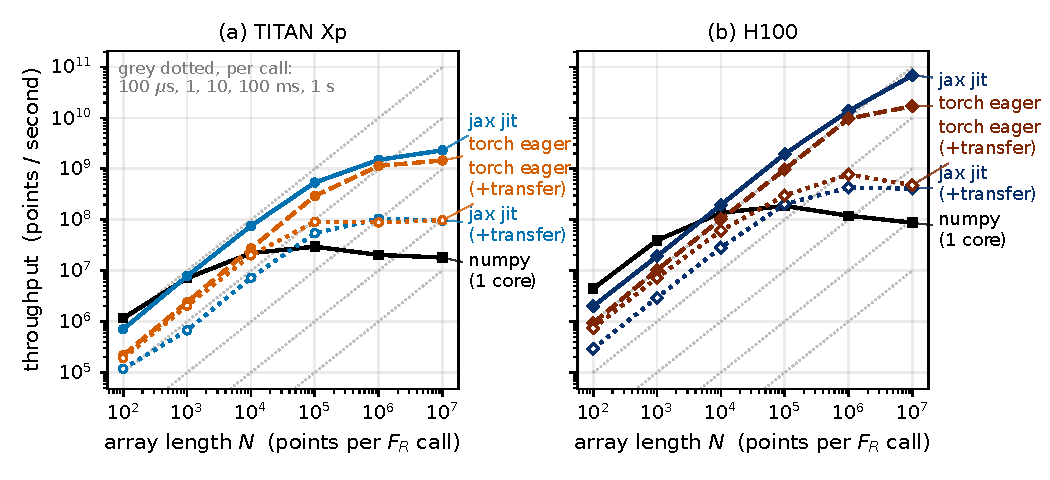
\includegraphics[width=0.48\textwidth,clip=]{../figures/g2_throughput/g2_throughput.pdf}
  \caption{Throughput of the radial force of a Plummer potential as a
    function of the number of points per call. The left panel shows the
    development machine, with \numpy\ on the CPU and \jax\ and \torch\
    on an NVIDIA TITAN~Xp; the right panel shows a node of the Trillium
    cluster, with an NVIDIA H100. Solid lines are compute-only, dashed
    lines include the transfer of inputs and outputs between host and
    device. Dotted lines mark constant wall time per call, which the GPU
    curves follow while launch-bound.}\label{fig:throughput}
\end{figure}
